\documentclass[12pt]{spieman} 
\usepackage{amsmath,amsfonts,amssymb}
\usepackage{graphicx}
\usepackage{setspace}
\usepackage{tocloft}

\title{Text Classification using Convolutional Neural Network}

\author[a]{Genqian Hu}
\affil[a]{George Mason University}

\renewcommand{\cftdotsep}{\cftnodots}
\cftpagenumbersoff{figure}
\cftpagenumbersoff{table}
\begin{document}
\maketitle

\begin{abstract}
This paper introduces Convolutional Neural Network briefly and applies it to a text classification task. According to the experimental results, trained CNN models are sensitive to the total number of categories from dataset. The performance gets worse considerably as there are more categories taken from dataset.
\end{abstract}

% Include a list of up to six keywords after the abstract
\keywords{text classification, word embedding, CNN, convolution}

\begin{spacing}{1.5}   % use double spacing for rest of manuscript

\section{Introduction}
The world is changing everyday rapidly in this century. So, there are countless news published on the Internet to let people keep track of what's happening today without leaving their hsect:introomes. But the news need to be assign a related category before they get published online. The problem is the news do not label themselves. And classifying them manually costs too much. Thus, automatic text classification is getting more and more important nowadays.
\newline
Convolutional neural network(CNN) has been doing an excellent job on image analysis, because CNN can extract high-level features from images to grasp the idea of them by the convolutional operation. However, there are just a few researches which apply CNN for text classification task in recent years.\cite{ref2} \cite{ref3}\cite{ref4} So, there is a need to test how CNN will perform on text classification.



\section{Solution}
For this text classification task, a CNN with 2 different shapes convolutional kernels is set up. For each kernel, activation function ReLu is applied to them. And a pooling layer is right after that. Finally, the outputs of each kernel will be connected and flattened. The category which has the largest value will be the predicted category by CNN. TensorFlow will operate back propagation automatically.
\newline
For a picture, each pixel of it has a grayscale channel or 3 RGB channels. So a picture can be transform into a matrix conveniently. And the size of the matrix is the size of the picture for a grayscale image. But if the input is a text file, there are some preprocessing tasks to do before the convolutional operations.


    \subsection{GloVe Word Embedding}
    A word embedding is a set like a dictionary in natural language processing, where each word is mapped to a unique vector. GloVe is an algorithm invented by Computer Science Department of Stanford University to represent a word by a vector. Instead of training my own word embeddings, I use a pre-trained word embedding which is the Glove.6B.50d which contains 400,000 words. This pre-trained word embedding is trained on Wikipedia. 6B denotes the number of tokens the data was trained on and 50d denotes the dimension of each vector. Figure 1 gives an example that each word is stored by a vector.
    \begin{figure}[h!]
    \centering
    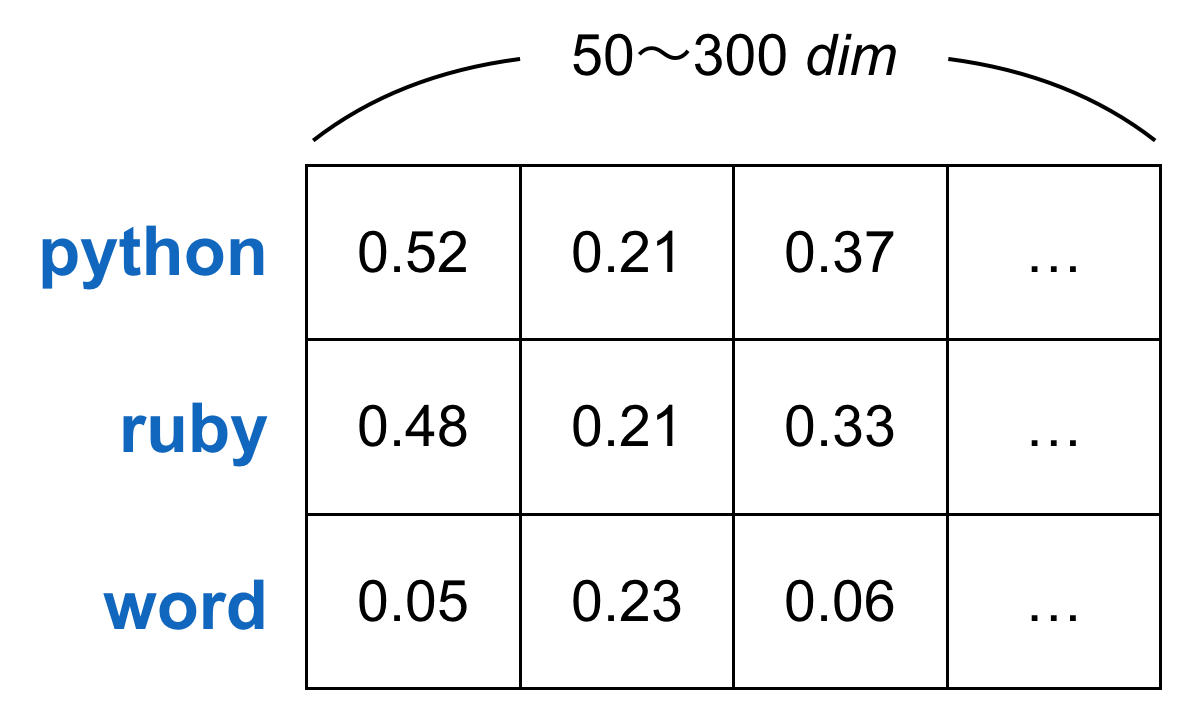
\includegraphics[width=0.80\textwidth]{figures/word_embedding.png}
    \caption{Word embedding}
    \label{threadsVsSync}
    \end{figure}

    \subsection{Convolutional Neural Network}
    Convolutional Neural Network is a kind of structure of artificial neural networks. And it has been well-known since Yann LeCun first successfully applied CNN structure on optical character recognition. And he is also considered as the founding person of the convolutional nets. Figure 2 is the structure of a famous CNN called LeNet for handwriting recognition\cite{ref1}.
    \begin{figure}[h!]
    \centering
    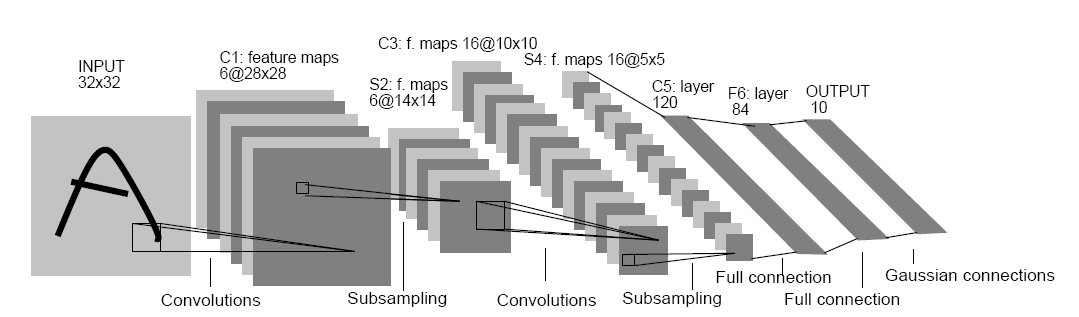
\includegraphics[width=0.80\textwidth]{figures/lenet.png}
    \caption{LeNet}
    \label{threadsVsSync}
    \end{figure}

        \subsubsection{Convolutional Layer}
        Convolutional layer is the core of a CNN as we can learn this easily from the connection of the name. At this layer, many kernels or filters are applied to the input matrices to compute the dot products between them during the forward propagation. After some training, each filter gets activated (the value of output is higher) when it detects a specific feature from input matrices. If CNN applies 2 3x3 filters with stride 1x1 to a 28x28 input matrix, the output will be a 26x26x2 matrix after the convolutional operation. Its dimension gets higher because there is a 26x26 output matrix for each filter.
        \subsubsection{Pooling Layer}
        Pooling layer is another important layer for a CNN. Max pooling is the most commonly used algorithm for this layer. Usually the shape of pooling is 2x2 which means for each 2x2 sub-matrix of the output matrix from previous layer, it takes the largest value from the 2x2 matrix as the output. Sometimes average pooling is used to get the average value of the sub-matrix. Figure 3 introduces the idea of max pooling and average pooling.
        \begin{figure}[h!]
        \centering
        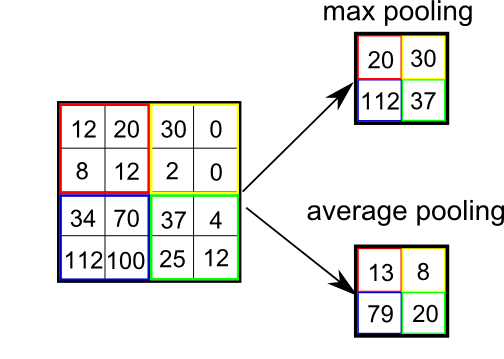
\includegraphics[width=0.80\textwidth]{figures/pooling.png}
        \caption{2 ways of pooling}
        \label{threadsVsSync}
        \end{figure}

        \subsubsection{Outstanding Features}
        Local connectivity and Weights sharing both are the advantages of CNN. Local connectivity refers to that each neuron is associated with a small region of the input and adjacent layers. So there are much less parameters to be updated when compared to fully connected for each neuron. And also, less parameters relieves the case of overfitting during the training step.
        In brief, each filter is an example for weight sharing. When scanning a picture with a filter, each part of this picture is scanned by the same filter, which means all parts of the picture share the same filter. This technique reduces the number of parameters as well.

    \subsection{Structure}
        \subsubsection{Embedding Layer}
        The first layer of the CNN on text classification for this paper is the embedding layer. At this layer, each word from the input dataset is mapped to a 50-dimensional vector by looking it up from the pre-trained GloVe word vector. The shape of the output matrix at this layer is [batch size, length of each data(1000), word embedding dimension, channels(1)].
        \subsubsection{Convolutional Layer}
        There are 2 shapes [5, word embedding dimension]  and [7, word embedding dimension] of filters at this layer. Each shape of filter contains 128 filters. So there are 2 branches here. For each input, the channels of shape will increase from 1 to 128.
        \subsubsection{ReLu Layer}
        Rectified Linear Unit(ReLu) is chosen here to add non-linearity  its derivative is a constant. So using ReLu can accelerate the training time. Figure 4 is how ReLu looks like.
        \begin{figure}[h!]
        \centering
        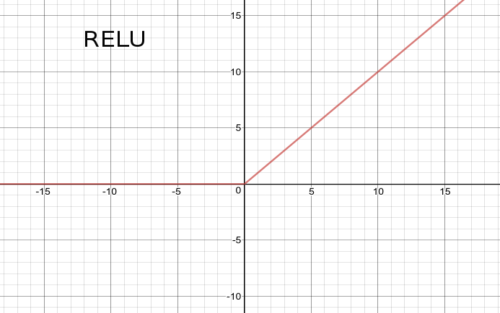
\includegraphics[width=0.80\textwidth]{figures/relu.png}
        \caption{ReLu activation function}
        \label{threadsVsSync}
        \end{figure}
        \subsubsection{Pooling Layer}
        Max pooling is applied at this layer. The pooling shape here is the same as the output from the previous layer for height and width. So, the size of the output is [batch size, 1, 1, number of each filters(128)] for both different branches of this CNN.
        \subsubsection{Concatenation and Flattening Layer}
        The outputs from previous layers of 2 branches are concatenated to a single matrix with size [batch size, 1, 1, total number of filters] here. And then it's flattened to a matrix with size [batch size(64), total number of filters(256)].
        \subsubsection{Predictions and Loss function}
        I just use argmax function to get the largest value so that the category with that value will be the predicted category. Or a softmax function can be applied here to get a normalized output.
        Cross entropy loss chosen here to compute the loss during each training step.
        \subsubsection{Dropout and Learning rate decay}
        Dropout is a regularization technique to avoid overfitting. It drops out some neurons randomly at each training step. For the CNN models of this paper, the value of dropout is 0.85 which means 15\% neurons are dropped out randomly for each training step.
        If the learning rate is fixed, convergence takes too long when learning rate is small or oscillate around some value when its too big. Learning rate decay makes the learning rate big so that it converges fast during the first several epochs of training. And the learning rate keeps decreasing to let the model get closer to the optimal model.

\section{Experiments}

    \subsection{Dataset}
    The dataset for training and testing the model is the 20newsgroup which consists of nearly 18846 news from 20 categories. Sci-kit has already split the dataset into a training and a testing set. The training set contains 11314 news. And the testing set contains 7532 news, which means the ratio of training set to testing set is roughly 6:4. Sklearn offers parameters to choose the categories from the all dataset conveniently.
    \subsection{Experimental setup}
        \subsubsection{Tensorflow}
        I use Tensorflow1.0 to implement the Convolutional Neural Network in python. TensorFlow is an open-source software library produced by Google Brain team for machine learning programming. It can operate the back propagation of neural networks intelligently so that programmer just need to set the forward propagation part. It has updated quickly. And each update introduces many new features but also changes some functions' names which means it has bad backward compatibility. The latest version is TensorFlow v1.40.
        \subsubsection{CUDA}
        Compute Unified Device Architecture(CUDA) is a parallel computing platform and application programming interface model produced by Nvidia. It supports TensorFlow to work on GPU so that the performance of TensorFlow is much better than working on CPU. I use CUDA 8.0 though the latest version is CUDA 9.0.
    \subsection{Experimental Results}
    The program were coded in python and executed on a desktop (Intel Core i7-6700K Processor, RAM 16 gigabyte, GTX 980 TI).

    \begin{table}
    \caption{Training time}
    \begin{center}
    \begin{tabular}{|l|l|l|}
    \hline
    \rule[-1ex]{0pt}{3.5ex}  Number of categories &CNN(50d)&CNN(100d)  \\
    \hline\hline
    \rule[-1ex]{0pt}{3.5ex}  3 &133s & 221s\\
    \hline
    \rule[-1ex]{0pt}{3.5ex}  5 &210s & 317s\\
    \hline
    \rule[-1ex]{0pt}{3.5ex}  10 &403s & 594s\\
    \hline
    \rule[-1ex]{0pt}{3.5ex}  15 &596s & 597s\\
    \hline
    \rule[-1ex]{0pt}{3.5ex}  20 &792s & 1138s\\
    \hline
    \end{tabular}
    \end{center}
    \end{table}

    \begin{table}
    \caption{Experimental results}
    \begin{center}
    \begin{tabular}{|l|l|l|l|l|}
    \hline
    \rule[-1ex]{0pt}{3.5ex}  Number of categories & Naive Bayes & SVM &CNN(50d)&CNN(100d)  \\
    \hline\hline
    \rule[-1ex]{0pt}{3.5ex}  3 &88\% & 92\%& 82\%& 81\%\\
    \hline
    \rule[-1ex]{0pt}{3.5ex}  5 &87\% & 92\%& 78\%& 79\%\\
    \hline
    \rule[-1ex]{0pt}{3.5ex}  10 &85\% & 86\%& 58\%& 61\%\\
    \hline
    \rule[-1ex]{0pt}{3.5ex}  15 &83\% & 88\%& 50\%& 60\%\\
    \hline
    \rule[-1ex]{0pt}{3.5ex}  20 &76\% & 82\%& 50\%& 53\%\\
    \hline
    \end{tabular}
    \end{center}
    \end{table}
    Both CNN models are trained with 64 batch size and 200 epochs. Table 1 shows that as the number of categories of dataset increases, the training time for both model go up linearly. The reason is that for different categories, they have nearly amount of news. And during preprocessing, each news is operated to take only the first 1000 words of them. So the processing time on each news should be roughly the same.
    \newline
    The CNN models are compared with SVM and Naive Bayes for different numbers of categories\cite{ref5}. The SVM is implemented by using a SGD classifier with loss equals to 'hinge'. For each comparison, same categories and data are applied for each model. Table 2 shows the result that SVM holds the best accuracy for each number of categories. Then Naive Bayes has the accuracy which is over 80 percent in most cases. Both CNN models' performance drop hugely when classifying news from over 5 groups. But the one using 100-dimensional pre-trained GloVe word embedding gets slightly better results. And considering SVM and Naive Bayes can finish the training instantly, a lot of time are spent on training the CNN models. And if a parameter or the structure is slightly changed, the model has to be training again.
    \subsection{Results Analysis}
    When the number of categories is more than 5, the accuracy of CNN models is much worse than the other 2 models. There are several potential reasons for this situation.
    \newline
    The filters of the convolutional layer can move both horizontally and vertically if the input file is an image. But for a text file, because each row of the matrix represent a single word, filters can't move horizontally or it would tear apart this word. So filters are only allowed to move vertically like operating on a 1-dimensional vector. Thus, convolution operation is weakened when dealing with sentences.
    \newline
    The GloVe pre-trained word embedding is trained on different dataset so that it doesn't fit the 20newsgroup dataset perfectly.
    \newline
    The CNN models are overfitting the training data though dropout is applied. According to the performance on the training set, the accuracy is always above 95 percent for each run.
    \subsection{Feature Works}
    Like a colorful picture consists RGB channels, a word can be represent by different word embedding algorithm. Then each sentence can be transformed into a 3dimensional matrix like a picture. Like a 5 words sentence can be transformed into a matrix wish shape [5,50,3]. [5,50,1] uses Word2Vec The other 2 use GloVe and one-hot. This should help CNN better grasp the feature of input text.
    \newline
    Other technique need to be deployed to avoid overfitting like getting more data and using early stopping. Or the percentage of dropout can be set higher.
    \newline
    Dataset can be loaded a portion each time instead of loading the whole dataset into the memory which may run out of it.
\section{Conclusion}
Convolutional neural network is a powerful tool for machine learning, but people will have to spend a lot of time on tuning the parameters, changing the structure and training the model. And CNN has been proved it's able to works well on text categorization by applying k-max-pooling to keep more features.cite{ref4} The performance of that CNN model is better than the SVM for some datasets. Thus, it's all about how to build a proper structure for a specific task. Or SVM can gives a relatively robust classifier for text classification.




\newpage
%%%%% References %%%%%
\begin{thebibliography}{99}
\bibitem{ref1}Y. Lecun, B. Boser, J. S. Denker, D. Henderson, R. E. Howard, W. Hubbard, and L. D. Jackel, ��Backpropagation Applied to Handwritten Zip Code Recognition,�� Neural Computation, vol. 1, no. 4, pp. 541�C551, 1989.
\bibitem{ref2}R. Johnson and T. Zhang, ��Effective Use of Word Order for Text Categorization with Convolutional Neural Networks,�� Proceedings of the 2015 Conference of the North American Chapter of the Association for Computational Linguistics: Human Language Technologies, 2015.
\bibitem{ref3}Y. Kim, ��Convolutional Neural Networks for Sentence Classification,�� Proceedings of the 2014 Conference on Empirical Methods in Natural Language Processing (EMNLP), 2014.
\bibitem{ref4}R. Johnson and T. Zhang, ��Effective Use of Word Order for Text Categorization with Convolutional Neural Networks,�� Proceedings of the 2015 Conference of the North American Chapter of the Association for Computational Linguistics: Human Language Technologies, 2015.
\bibitem{ref5}C. Wirawan, https://github.com/cahya-wirawan/ML-Collection
\end{thebibliography}


\end{spacing}
\end{document}
